% !TeX root = ../main.tex
% !TeX root = ../main.tex
% Add the above to each chapter to make compiling the PDF easier in some editors.

\chapter{Fundamentals of TUM-Live}\label{chapter:fundamentals}

\section{GoCast Lecture Streaming Service}

\subsection{Overview}
GoCast is a fully self-hosted platform for live streaming and recording of lectures developed by students at \ac{TUM}. The source code is open-source, accessible at \href{https://github.com/TUM-Dev/gocast}{github.com/TUM-Dev/gocast} and licensed under the MIT license. Its main features include:

\begin{itemize}
    \item Automatic live streaming from auditoriums based on lecture schedules imported from CAMPUSonline (campus management system used at \ac{TUM} as TUMOnline).
    \item Self-service interface for lecturers to schedule and manage their \ac{VOD}s and streams.
    \item Automated import of lecture schedules and enrollments from CAMPUSonline.
    \item Self-streaming via third party streaming software such as \href{https://obsproject.com}{OBS}\footnote{\url{https://obsproject.com}}, \href{https://zoom.us}{Zoom}\footnote{\url{https://zoom.us}}, etc.
    \item Automatic recording of live streams.
    \item Manual \ac{VOD} uploads.
    \item Automatic post-processing of recordings.
    \begin{itemize}
        \item Detect silence in videos and makes them skip-able.
        \item Transcribe live streams and \ac{VOD}s using the \href{https://github.com/openai/whisper}{Whisper LLM}\footnote{\url{https://github.com/openai/whisper}}.
        \item Generate thumbnails.
    \end{itemize}
    \item Optional live chat for viewers to ask questions.
    \begin{itemize}
        \item Polls can be created by lecturers.
        \item Questions can be upvoted by viewers and answered or hidden by lecturers.
        \item Optional moderation features for lecturers.
    \end{itemize}
\end{itemize}

\subsection{Current System Architecture}

\begin{figure}[htpb]
    \centering
    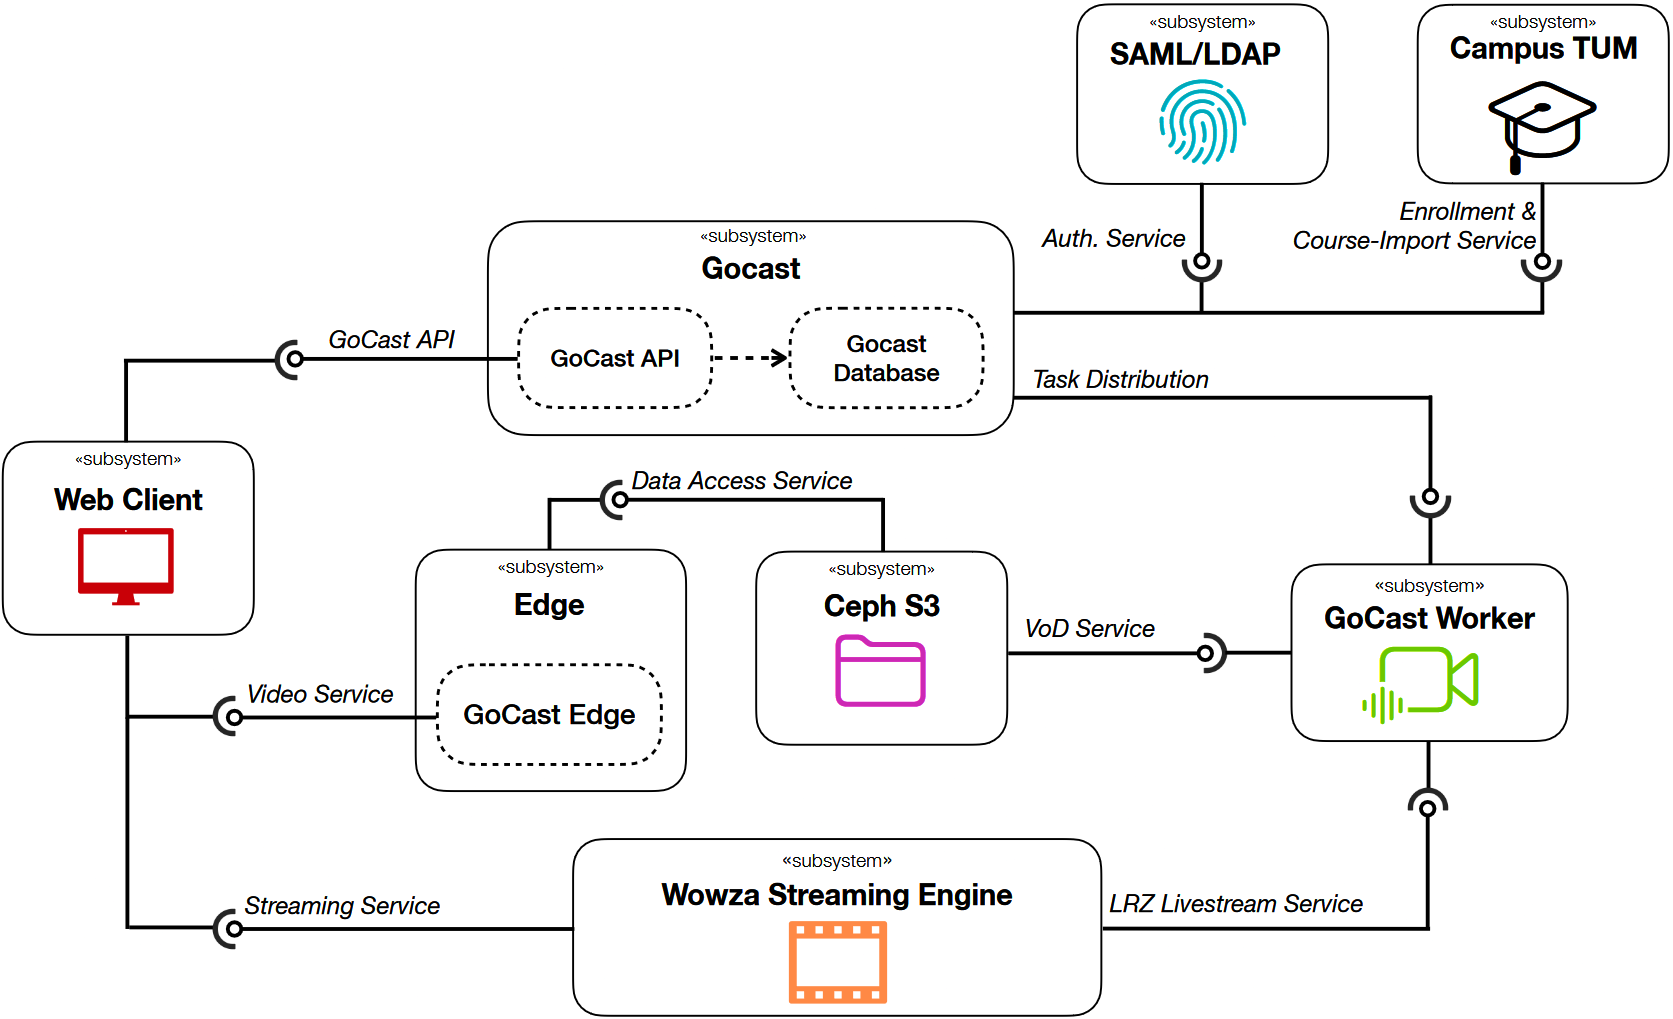
\includegraphics[width=\linewidth]{images/ssd-new.png}
    \caption[System Architecture of GoCast]{System Architecture of GoCast}\label{fig:old-system-architecture}
\end{figure}

The current system architecture of GoCast can be divided into three parts:

\subsubsection{1. User-, course- and task-management:}
At the core of the GoCast system, there is the main \ac{API} built on the \href{https://github.com/gin-gonic/gin}{Gin-Gonic}\footnote{\url{https://github.com/gin-gonic}} Framework and connected to a \href{https://mariadb.org}{MariaDB}\footnote{\url{https://mariadb.org}} Database. Its main functionality is to manage users, courses, streams, pull events from CAMPUSonline and schedule tasks. For user authentication, it can use \ac{SSO} and \ac{SAML} to allow users to authenticate themselves with their university credentials.

\subsubsection{2. \ac{VOD} upload related components:}
Next, whenever a lecture is uploaded as a VOD, the video data is sent to a Worker which then transcodes and segments the video into MPEG-2 compressed video transport stream files using \href{https://ffmpeg.org/}{FFmpeg}\footnote{\url{https://ffmpeg.org}}. These segments are then copied to a shared storage using the VOD Service component so that they can then later be distributed by the Edge Server to the end-user.
Currently there are plans to replace the Worker subsystem with a more robust and efficient Runner system. However, as the Runner is still in the development phase and not tested yet (see \autoref{subsection:runner}), we will mainly refer to the Worker subsystem throughout this thesis (although in principle the Worker and Runner concepts can be used interchangeably).

\subsubsection{3. Lecture recording and live streaming:}
Lastly, for live streaming GoCast depends on external streaming infrastructure. In \ac{TUM}'s case this is the live streaming infrastructure of the \ac{LRZ} which internally runs the \href{https://doku.lrz.de/allgemeines-526418642.html}{Wowza Streaming Engine}\footnote{\url{https://doku.lrz.de/allgemeines-526418642.html}}. Whenever a lecturer starts a live stream from a lecture hall, the produced \ac{RTMP} stream is sent via the Worker to the \ac{LRZ} streaming service which then processes the live stream and makes it available for the viewer in real-time. When the viewer now watches a live stream, the video is streamed directly to the user's browser client from the \ac{LRZ} streaming service. 

\section{TUM-Live}

GoCast is in use at the \ac{TUM} as \href{https://tum.live}{TUM-Live}. This section aims to group and structure existing information related to TUM-Live's history, technical setup and statistics in a concise manner. 

\subsection{Technical Setup of TUM-Live}

To professionally stream hundreds of lectures every semester, TUM-Live has integrated GoCast in a complex infrastructure of hardware components deployed in separated VLANs that allow for easy streaming from a lecture hall without having to do additional configuration at the beginning of each lecture. 
First, there needs to be at least one pan–tilt–zoom camera equipped in a lecture hall to record and follow the lecturer as well as the white-/blackboard.
Then, every lecture hall needs to be equipped with a so called \href{https://www.extron.com/article/smp}{\ac{SMP}}\footnote{\url{https://www.extron.com/article/smp}} which is an all-in-one recording and streaming processor that captures, switches, scales and distributes audio and video sources and presentations. In addition to that, it also provides multiple concurrent streams including flexible two-window layouts and full screen views. This is especially useful as it allows sending video data in three different formats to the main TUM-Live instance: \texttt{CAM} for the camera pointing at the lecturer, \texttt{PRES} for the currently shown screen of the lecturer's laptop or \texttt{COMB} for a two-window view of both. The \ac{SMP} can also be used as a backup device for the \ac{VOD} in case something goes wrong in a later stage (e.g., a Worker has an outage and the recorded stream is "lost") as the \ac{SMP} device creates a local copy of the recording. The main problem with \ac{SMP}s is their high cost, as one device can cost more than 10,000 EUR.

\subsection{Progress of TUM-Live}

Originally, TUM-Live was started in 2019 by the multimedia group of the former faculty of informatics to stream overcrowded lectures of popular courses into different lecture halls as some courses had more students than lecture hall seats. A lecturer would create a RTMP stream of his current lecture and publish the stream in a private network to a different lecture hall which then would display the streams to the students. At the same time this system started being used more and more to provide a public live stream and \ac{VOD} portal and archive for students of selected courses. The system itself was - in comparison to the current system - rather simple as it displayed a list of streams\footnote{\url{https://web.archive.org/web/20191001114650/https://live.rbg.tum.de}} that would show the currently live stream or link to uploaded .mp4 files.
This quickly changed in 2020 as the COVID-19 pandemic created a high demand for online lecture video streams, which then resulted in the development of GoCast. Starting from fall 2021, the old TUM-Live system switched to using GoCast, as provided a user friendly and easily accessible user interface for students and a cost-efficient and privacy-focused alternative to other lecture streaming platforms for \ac{TUM}'s media group "ProLehre". 

Nowadays TUM-Live offers live and on-demand videos of lectures and events from \ac{TUM}'s \href{https://www.cit.tum.de}{\ac{CIT}}\footnote{\url{https://www.cit.tum.de}}. Some of \ac{TUM}'s other schools have also shown interest in joining the \ac{CIT} in using TUM-Live, but do not have the budget to equip all lecture halls with \ac{SMP}s. However, this issue might soon be resolved, as a student has developed his own open-source \ac{SMP} called \ac{VMP} that aims to re-implement the functionality of the \ac{SMP} in software, using the \href{https://gstreamer.freedesktop.org/}{GStreamer Multimedia Framework}\footnote{\url{https://gstreamer.freedesktop.org/}}. The target hardware is a small single-board computer with accelerated Multimedia encoding/decoding and additional HDMI capture capabilities which costs only around 500 EUR. Given the low cost of such a device, it is very likely that other \ac{TUM} schools and possible even other universities will join TUM-Live in the future.

\subsection{User Statistics of TUM-Live}\label{subsection:user-stats-tumlive}

Since its creation in February of 2021, TUM-Live has been used to stream thousands of hours of video every semester for more than 1,300 courses, 20,000 streams and 30,000 students. The following plots (see \autoref{fig:tumlive-stats}) display a broad overview of viewer metrics from the current system. As the \textit{VoD activity throughout the day} plot shows, the hours at which the users watch recorded \ac{VOD}s is normally distributed, with the mean being around 4PM. Most students use TUM-Live throughout the entire lecture week (see \textit{VoD activity per day of week} plot showing an evenly distributed \ac{VOD} activity over the week), meaning that the Edge Servers need to be fully functional at all times. At its peak, there are nearly 6,000 \ac{VOD} replays per day (see \textit{VoD activity per day}) - while at times - mostly during the semester breaks - there are weeks with nearly no \ac{VOD} activity at all.

\begin{figure}[htpb]
    \centering
    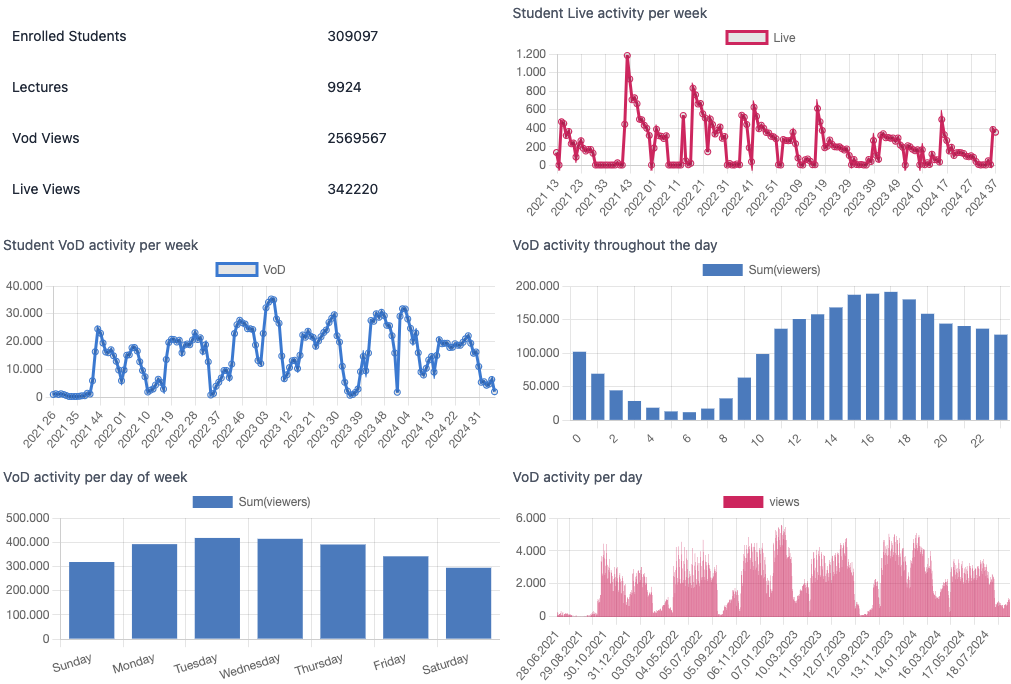
\includegraphics[width=\linewidth]{images/TUMLiveStats.png}
    \caption[TUM-Live Statistics]{TUM-Live Viewing Statistics}\label{fig:tumlive-stats}
\end{figure}

What's especially interesting is the development of the number of users, courses and streams over time. As can be seen in \autoref{fig:tumlive-stats-2}, at the beginning of each semester there is a clear spike in new users, created courses and streams. This is mainly due to the automatic import of lecture data and enrollments from CAMPUSonline. Between semesters, the increase in new users and courses is rather flat, with a slight increase in the number of streams (mostly streams that have been created manually).  

\begin{figure}[htpb]
    \centering
    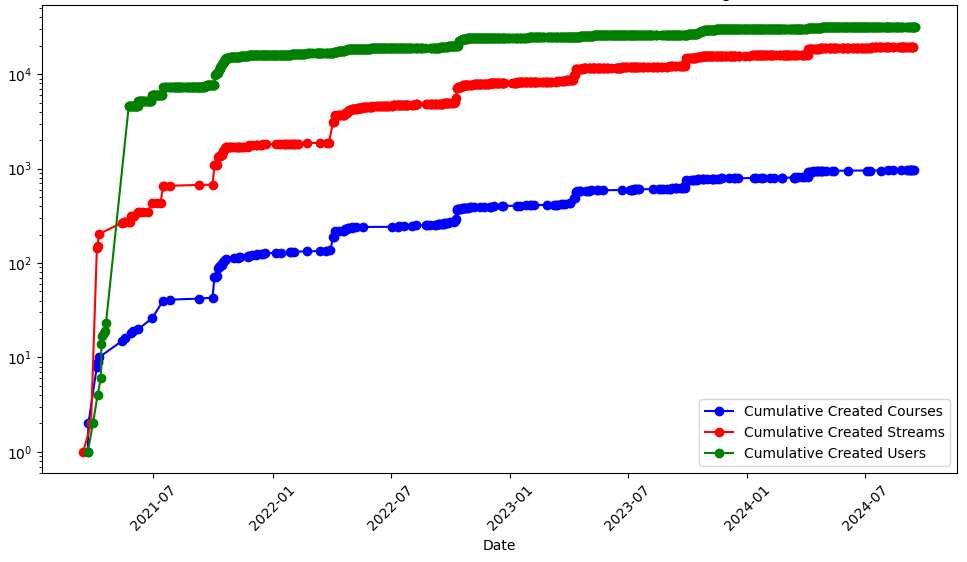
\includegraphics[width=\linewidth]{images/TUMLiveStats2.png}
    \caption[Cumulative Number of Users, Courses and Streams over Time (Log Scale)]{Cumulative Number of Users, Courses and Streams over Time (Log Scale)}\label{fig:tumlive-stats-2}
\end{figure}
